\documentclass[11pt,a4paper]{article}
\usepackage[utf8]{inputenc}
\usepackage[T1]{fontenc}
\usepackage{amsmath,amssymb,amsthm}
\usepackage{mathtools}
\usepackage{geometry}
\usepackage{hyperref}
\usepackage{cleveref}
\usepackage{booktabs}
\usepackage{array}
\usepackage{longtable}
\usepackage{tikz}
\usetikzlibrary{arrows.meta,positioning,shapes.geometric,calc,decorations.pathmorphing}
\usepackage{tcolorbox}
\tcbuselibrary{theorems,skins,breakable}
\usepackage{xcolor}
\usepackage{enumitem}

\geometry{margin=1in}

\hypersetup{
    colorlinks=true,
    linkcolor=blue!70!black,
    citecolor=green!50!black,
    urlcolor=blue!70!black
}

% Theorem environments
\newtheorem{theorem}{Theorem}[section]
\newtheorem{lemma}[theorem]{Lemma}
\newtheorem{proposition}[theorem]{Proposition}
\newtheorem{corollary}[theorem]{Corollary}
\newtheorem{definition}[theorem]{Definition}
\newtheorem{remark}[theorem]{Remark}

% Boxes
\newtcolorbox{resultbox}[1][]{
    colback=blue!5!white,
    colframe=blue!75!black,
    fonttitle=\bfseries,
    title=#1,
    breakable
}

\newtcolorbox{designrule}[1][]{
    colback=orange!5!white,
    colframe=orange!75!black,
    fonttitle=\bfseries,
    title=Design Rule,
    breakable
}

\newtcolorbox{openbox}[1][]{
    colback=red!5!white,
    colframe=red!75!black,
    fonttitle=\bfseries,
    title=Open Item,
    breakable
}

% Epistemic tags
\newcommand{\tagD}{\textcolor{blue!70!black}{[D]}}
\newcommand{\tagDc}{\textcolor{blue!50!black}{[Dc]}}
\newcommand{\tagP}{\textcolor{green!50!black}{[P]}}
\newcommand{\tagI}{\textcolor{gray}{[I]}}
\newcommand{\tagBL}{\textcolor{purple}{[BL]}}
\newcommand{\tagOPEN}{\textcolor{red!70!black}{[OPEN]}}

% Math operators
\DeclareMathOperator{\Tr}{Tr}
\DeclareMathOperator{\diag}{diag}
\DeclareMathOperator{\rank}{rank}
\DeclareMathOperator{\ad}{ad}

\title{\textbf{Derivation v35: GUT BC Survivor Map} \\[0.5em]
\large Boundary Condition Selection of Residual Gauge Symmetry \\
in 5D $\to$ 4D Dimensional Reduction}
\author{EDC Block-003 Program}
\date{February 2026}

\begin{document}

\maketitle

\begin{abstract}
We derive the general mechanism by which boundary conditions (BCs) in 5D gauge
theories select the residual 4D gauge group. The ``survivor rule'' establishes
that gauge generators with Neumann/Neumann BCs (or orbifold parity $(+,+)$)
retain massless zero-modes, while Dirichlet or $(-)$ parity removes them.
We apply this to four GUT tracks---SU(5), SO(10), Pati--Salam, and $E_6$---providing
explicit parity matrices $(P_0, P_L)$ that break each parent group to the
Standard Model $SU(3)_c \times SU(2)_L \times U(1)_Y$. A survivor/broken
generator census, scale regime map, matter parity stub, and BC$\to$Breaking
dictionary complete the structural analysis. \textbf{No forbidden numerical
inputs} (electroweak masses, Planck scale, fine-structure constant) appear
anywhere in this derivation.
\end{abstract}

\tableofcontents
\newpage

%=============================================================================
\section{Reader Contract}
%=============================================================================

\subsection{Epistemic Tags}
\begin{itemize}[leftmargin=2cm]
    \item[\tagD] \textbf{Derived}: follows from stated axioms/postulates
    \item[\tagDc] \textbf{Derived with convention}: choice of normalization/phase
    \item[\tagP] \textbf{Postulate}: starting assumption
    \item[\tagI] \textbf{Identity}: mathematical fact
    \item[\tagBL] \textbf{Borrowed from literature}: standard result
    \item[\tagOPEN] \textbf{Open}: requires further work
\end{itemize}

\subsection{Scope}
This derivation establishes:
\begin{enumerate}
    \item The \textbf{survivor rule}: which gauge generators retain 4D zero-modes
    \item The \textbf{projector algebra}: how parities define the residual subalgebra
    \item \textbf{Four GUT tracks}: explicit BC patterns for SM emergence
    \item \textbf{Matter consistency}: chirality requirements for fermions
    \item \textbf{BC$\to$Breaking dictionary}: what must be N vs D
\end{enumerate}

\subsection{What is NOT Derived}
\begin{itemize}
    \item Numerical gauge couplings or unification scales
    \item Running or threshold corrections
    \item Complete matter spectra or Yukawa matrices
    \item Anomaly cancellation (noted as \tagOPEN)
\end{itemize}

%=============================================================================
\section{5D Gauge Theory Setup}
%=============================================================================

\subsection{Action and Field Content}

Consider a 5D gauge theory with gauge group $G$ on the interval $y \in [0, L]$
or orbifold $S^1/\mathbb{Z}_2$. \tagP

\begin{equation}
\label{eq:5D-action}
S_{\text{gauge}} = -\frac{1}{4g_5^2} \int d^4x \int_0^L dy \sqrt{-G}\,
F_{MN}^a F^{MN,a}
\end{equation}

where $M, N \in \{0,1,2,3,5\}$ and $a$ runs over generators of $\mathfrak{g} = \text{Lie}(G)$. \tagP

The 5D gauge field decomposes as:
\begin{equation}
\label{eq:AM-decomp}
A_M^a = (A_\mu^a, A_5^a), \quad \mu = 0,1,2,3
\end{equation}

\subsection{Field Strength Components}

The 5D field strength has components:
\begin{align}
\label{eq:Fmunu}
F_{\mu\nu}^a &= \partial_\mu A_\nu^a - \partial_\nu A_\mu^a + f^{abc} A_\mu^b A_\nu^c \\
\label{eq:Fmu5}
F_{\mu 5}^a &= \partial_\mu A_5^a - \partial_5 A_\mu^a + f^{abc} A_\mu^b A_5^c
\end{align}

where $f^{abc}$ are the structure constants: $[T^a, T^b] = i f^{abc} T^c$. \tagI

%=============================================================================
\section{Boundary Conditions: The Survivor Rule}
%=============================================================================

\subsection{Variational Principle}

Varying the action \eqref{eq:5D-action} with respect to $A_\mu^a$ yields:
\begin{equation}
\label{eq:variation}
\delta S \supset \int d^4x \left[ F^{a}_{\mu 5} \delta A^{a,\mu} \right]_{y=0}^{y=L}
\end{equation}

For the boundary term to vanish, we need \textbf{either}: \tagD
\begin{align}
\label{eq:neumann-bc}
\text{Neumann (N):} \quad & \partial_5 A_\mu^a \big|_{y=0,L} = 0 \\
\label{eq:dirichlet-bc}
\text{Dirichlet (D):} \quad & A_\mu^a \big|_{y=0,L} = 0
\end{align}

\subsection{BC Registry for Gauge Fields}

\begin{definition}[BC Registry]
\label{def:bc-registry}
For each generator $T^a$, assign boundary conditions at $y=0$ and $y=L$:
\begin{equation}
\label{eq:bc-pair}
\text{BC}(A_\mu^a) = (\text{BC}_0, \text{BC}_L) \in \{N, D\}^2
\end{equation}
The four possibilities are: $(N,N)$, $(N,D)$, $(D,N)$, $(D,D)$. \tagD
\end{definition}

\subsection{Mode Equation and Spectrum}

For $A_\mu^a(x,y) = \sum_n A_\mu^{a,(n)}(x) f_n^a(y)$, the profile satisfies:
\begin{equation}
\label{eq:mode-eq}
-\partial_5^2 f_n^a(y) = m_n^2 f_n^a(y)
\end{equation}

\begin{lemma}[Neumann Zero-Mode]
\label{lem:neumann-zero}
With BC $(N,N)$, there exists a constant zero-mode:
\begin{equation}
\label{eq:zero-mode-NN}
f_0(y) = \frac{1}{\sqrt{L}}, \quad m_0 = 0
\end{equation}
\end{lemma}

\begin{proof}
The general solution to \eqref{eq:mode-eq} with $m^2 = 0$ is $f(y) = A + By$.
Neumann at $y=0$: $\partial_5 f|_0 = B = 0$.
Neumann at $y=L$: $\partial_5 f|_L = B = 0$.
Both satisfied with $f = A = \text{const}$. Normalization gives $A = 1/\sqrt{L}$. \tagD
\end{proof}

\begin{lemma}[Dirichlet Excludes Zero-Mode]
\label{lem:dirichlet-no-zero}
With BC $(D,D)$, $(D,N)$, or $(N,D)$, there is \textbf{no} zero-mode.
\end{lemma}

\begin{proof}
For $m = 0$, $f(y) = A + By$.
\begin{itemize}
    \item $(D,D)$: $f(0) = A = 0$ and $f(L) = BL = 0 \Rightarrow B = 0$. Only $f \equiv 0$.
    \item $(D,N)$: $f(0) = A = 0$ and $\partial_5 f|_L = B = 0$. Only $f \equiv 0$.
    \item $(N,D)$: $\partial_5 f|_0 = B = 0$ and $f(L) = A = 0$. Only $f \equiv 0$.
\end{itemize}
No normalizable zero-mode exists. \tagD
\end{proof}

\begin{resultbox}[Survivor Rule]
\begin{theorem}[Zero-Mode Existence]
\label{thm:survivor}
A gauge generator $T^a \in \mathfrak{g}$ has a massless 4D gauge boson
(zero-mode) if and only if:
\begin{equation}
\label{eq:survivor-rule}
\boxed{\text{BC}(A_\mu^a) = (N, N)}
\end{equation}
Generators with any Dirichlet boundary are ``broken'' (no zero-mode). \tagD
\end{theorem}
\end{resultbox}

\subsection{Massive KK Tower}

For $(N,N)$ boundary conditions:
\begin{equation}
\label{eq:kk-NN}
f_n(y) = \sqrt{\frac{2}{L}} \cos\left(\frac{n\pi y}{L}\right), \quad
m_n = \frac{n\pi}{L}, \quad n \geq 1
\end{equation}

For $(D,D)$ boundary conditions:
\begin{equation}
\label{eq:kk-DD}
f_n(y) = \sqrt{\frac{2}{L}} \sin\left(\frac{n\pi y}{L}\right), \quad
m_n = \frac{n\pi}{L}, \quad n \geq 1
\end{equation}

For mixed $(N,D)$ or $(D,N)$:
\begin{equation}
\label{eq:kk-mixed}
m_n = \frac{(n + \tfrac{1}{2})\pi}{L}, \quad n \geq 0
\end{equation}

The lightest mode for mixed BC has mass $\pi/(2L)$, not zero. \tagD

%=============================================================================
\section{Orbifold Parities and Projectors}
%=============================================================================

\subsection{$S^1/\mathbb{Z}_2$ Orbifold}

Consider $S^1$ with $y \sim y + 2L$ and $\mathbb{Z}_2$ identification $y \sim -y$.
Fixed points are $y = 0$ and $y = L$. \tagP

Under the $\mathbb{Z}_2$ action at $y = 0$:
\begin{equation}
\label{eq:z2-action-0}
A_\mu(x, -y) = P_0 A_\mu(x, y) P_0^{-1}
\end{equation}

where $P_0$ is an automorphism of $G$ acting in the adjoint representation. \tagP

\subsection{Parity Matrix Action on Generators}

In components:
\begin{equation}
\label{eq:parity-components}
A_\mu^a(x, -y) = (P_0)^a{}_b A_\mu^b(x, y)
\end{equation}

Since $P_0^2 = \mathbf{1}$ (orbifold involution), eigenvalues are $\pm 1$:
\begin{equation}
\label{eq:parity-eigenvalue}
P_0 T^a P_0^{-1} = \eta_0^a T^a, \quad \eta_0^a \in \{+1, -1\}
\end{equation}

\begin{definition}[Parity Assignment]
\label{def:parity}
Each generator $T^a$ has parities $(\eta_0^a, \eta_L^a)$ at the two fixed points:
\begin{align}
\label{eq:parity-0}
P_0 T^a P_0^{-1} &= \eta_0^a T^a \\
\label{eq:parity-L}
P_L T^a P_L^{-1} &= \eta_L^a T^a
\end{align}
where $\eta \in \{+, -\}$. \tagDc
\end{definition}

\subsection{Parity$\leftrightarrow$BC Correspondence}

\begin{proposition}[Parity to BC Map]
\label{prop:parity-bc}
The orbifold parity assignment maps to interval BCs:
\begin{align}
\label{eq:parity-N}
\eta = + \quad &\Leftrightarrow \quad \text{Neumann} \\
\label{eq:parity-D}
\eta = - \quad &\Leftrightarrow \quad \text{Dirichlet}
\end{align}
\end{proposition}

\begin{proof}
For $\eta_0 = +$: $A_\mu(x, -y) = A_\mu(x, y)$ near $y = 0$, so
$\partial_5 A_\mu|_{y=0} = 0$ (Neumann).

For $\eta_0 = -$: $A_\mu(x, -y) = -A_\mu(x, y)$, so $A_\mu(x, 0) = 0$ (Dirichlet). \tagD
\end{proof}

\begin{corollary}[Survivor Rule, Orbifold Version]
\label{cor:survivor-orbifold}
\begin{equation}
\label{eq:survivor-orbifold}
\boxed{\text{Zero-mode exists} \quad \Leftrightarrow \quad (\eta_0, \eta_L) = (+, +)}
\end{equation}
\end{corollary}

%=============================================================================
\section{Projector Algebra: Survivor Subalgebra}
%=============================================================================

\subsection{Derivation of $\mathfrak{g}^{(+,+)}$}

\begin{theorem}[Survivor Algebra]
\label{thm:survivor-algebra}
The residual gauge algebra after BC/parity projection is:
\begin{equation}
\label{eq:survivor-algebra}
\boxed{\mathfrak{h} = \mathfrak{g}^{(+,+)} =
\{T \in \mathfrak{g} \mid P_0 T P_0^{-1} = +T,\; P_L T P_L^{-1} = +T\}}
\end{equation}
The corresponding Lie group $H$ is the 4D residual gauge group. \tagD
\end{theorem}

\begin{proof}
From Corollary \ref{cor:survivor-orbifold}, only generators with $(+,+)$ parity
have zero-modes. These form a closed subalgebra:
\begin{itemize}
    \item If $P_0 T^a P_0^{-1} = T^a$ and $P_0 T^b P_0^{-1} = T^b$, then
    $P_0 [T^a, T^b] P_0^{-1} = [T^a, T^b]$ (commutator of $(+)$ elements is $(+)$).
    \item Similarly for $P_L$.
\end{itemize}
Thus $\mathfrak{g}^{(+,+)}$ is a Lie subalgebra. \tagD
\end{proof}

\subsection{Dimension Counting}

\begin{proposition}[Generator Census]
\label{prop:gen-count}
Let $\dim \mathfrak{g} = N_G$. Partition into:
\begin{align}
\label{eq:n++}
N_{++} &= \#\{T^a : (\eta_0^a, \eta_L^a) = (+,+)\} \\
\label{eq:n+-}
N_{+-} &= \#\{T^a : (\eta_0^a, \eta_L^a) = (+,-)\} \\
\label{eq:n-+}
N_{-+} &= \#\{T^a : (\eta_0^a, \eta_L^a) = (-,+)\} \\
\label{eq:n--}
N_{--} &= \#\{T^a : (\eta_0^a, \eta_L^a) = (-,-)\}
\end{align}
Then:
\begin{equation}
\label{eq:dim-sum}
N_G = N_{++} + N_{+-} + N_{-+} + N_{--}
\end{equation}
and $\dim \mathfrak{h} = N_{++}$. \tagI
\end{proposition}

\subsection{Rank Preservation}

\begin{proposition}[Rank Under BC Breaking]
\label{prop:rank}
If both $P_0$ and $P_L$ are inner automorphisms (conjugation by group elements),
then $\rank(\mathfrak{h}) = \rank(\mathfrak{g})$. If either is an outer automorphism,
rank may decrease. \tagBL
\end{proposition}

For Standard Model emergence from GUTs:
\begin{equation}
\label{eq:sm-rank}
\rank(SU(3)_c \times SU(2)_L \times U(1)_Y) = 2 + 1 + 1 = 4
\end{equation}

This constrains which parent groups can break to SM:
\begin{equation}
\label{eq:rank-constraint}
\rank(G) \geq 4 \quad \text{(necessary)}
\end{equation}

%=============================================================================
\section{Track 1: SU(5)}
%=============================================================================

\subsection{Group Theory Data}

\begin{align}
\label{eq:su5-dim}
G &= SU(5), \quad \dim \mathfrak{su}(5) = 24, \quad \rank = 4 \\
\label{eq:su5-target}
H &= SU(3)_c \times SU(2)_L \times U(1)_Y, \quad \dim = 8 + 3 + 1 = 12
\end{align}

\subsection{Standard Parity Matrices}

The SU(5) generators in the fundamental representation are $5 \times 5$
traceless Hermitian matrices. \tagBL

\begin{definition}[SU(5) Parity]
\label{def:su5-parity}
Choose: \tagDc
\begin{equation}
\label{eq:su5-P0}
P_0 = P_L = \diag(+1, +1, +1, -1, -1)
\end{equation}
\end{definition}

Under conjugation by $P$:
\begin{align}
\label{eq:su5-block}
T = \begin{pmatrix} A_{3\times 3} & B_{3\times 2} \\ B^\dagger_{2\times 3} & C_{2\times 2} \end{pmatrix}
\quad \Rightarrow \quad
P T P^{-1} = \begin{pmatrix} A & -B \\ -B^\dagger & C \end{pmatrix}
\end{align}

\begin{proposition}[SU(5) Survivor Census]
\label{prop:su5-census}
With $P_0 = P_L = P$:
\begin{align}
\label{eq:su5-survivors}
(+,+): \quad & SU(3)_c \oplus SU(2)_L \oplus U(1)_Y \quad (8 + 3 + 1 = 12) \\
\label{eq:su5-broken}
(-,-): \quad & X, Y \text{ bosons} \quad (12 \text{ generators})
\end{align}
\end{proposition}

\begin{proof}
Diagonal blocks $A$ (traceless $3\times 3$) and $C$ (traceless $2\times 2$)
have $P T P^{-1} = T$, giving $SU(3)$ and $SU(2)$.
Off-diagonal $B$ has $P T P^{-1} = -T$, giving the 12 broken $X, Y$ generators.
The $U(1)_Y$ generator is $Y = \diag(1,1,1,-3/2,-3/2)/\sqrt{15}$
(or normalized convention), which commutes with $P$. \tagD
\end{proof}

\subsection{SU(5) Survivor Table}

\begin{table}[h]
\centering
\begin{tabular}{lcccc}
\toprule
Sector & Parity $(\eta_0,\eta_L)$ & Generators & Count & Status \\
\midrule
$SU(3)_c$ & $(+,+)$ & $\lambda_1, \ldots, \lambda_8$ & 8 & Survivor \\
$SU(2)_L$ & $(+,+)$ & $\sigma_1, \sigma_2, \sigma_3$ & 3 & Survivor \\
$U(1)_Y$ & $(+,+)$ & $Y$ & 1 & Survivor \\
$X$ bosons & $(-,-)$ & $T^{X_i}$ & 6 & Broken \\
$Y$ bosons & $(-,-)$ & $T^{Y_i}$ & 6 & Broken \\
\midrule
\textbf{Total} & & & \textbf{24} & \\
\bottomrule
\end{tabular}
\caption{SU(5) generator census under BC breaking.}
\label{tab:su5}
\end{table}

\subsection{Hypercharge Embedding}

In SU(5), hypercharge is embedded as: \tagBL
\begin{equation}
\label{eq:su5-Y}
Y = \frac{1}{\sqrt{60}} \diag(2, 2, 2, -3, -3)
\end{equation}

(with GUT normalization $\Tr(Y^2) = 1/2$). The SM normalization differs by
$\sqrt{3/5}$:
\begin{equation}
\label{eq:Y-normalization}
Y_{\text{SM}} = \sqrt{\frac{3}{5}} Y_{\text{GUT}}
\end{equation}

%=============================================================================
\section{Track 2: SO(10)}
%=============================================================================

\subsection{Group Theory Data}

\begin{align}
\label{eq:so10-dim}
G &= SO(10), \quad \dim \mathfrak{so}(10) = 45, \quad \rank = 5 \\
\label{eq:so10-target}
H &= SU(3)_c \times SU(2)_L \times U(1)_Y, \quad \dim = 12
\end{align}

SO(10) has rank 5 > 4, so one $U(1)$ factor must be broken. \tagI

\subsection{Breaking Chain Options}

SO(10) can break to SM through intermediate stages: \tagBL
\begin{align}
\label{eq:so10-ps}
SO(10) &\to SU(4)_C \times SU(2)_L \times SU(2)_R \to \text{SM} \\
\label{eq:so10-su5}
SO(10) &\to SU(5) \times U(1)_X \to \text{SM} \\
\label{eq:so10-direct}
SO(10) &\to \text{SM} \times U(1)_{B-L} \to \text{SM}
\end{align}

\subsection{Direct SO(10) $\to$ SM Breaking}

\begin{definition}[SO(10) Parity Matrices]
\label{def:so10-parity}
Using the spinor representation embedding, choose: \tagDc
\begin{align}
\label{eq:so10-P0}
P_0 &= \diag(\underbrace{+1}_{5}, \underbrace{-1}_{5}) \quad \text{(in 10-dim vector)} \\
\label{eq:so10-PL}
P_L &= \diag(+1,+1,+1,-1,-1,+1,+1,+1,-1,-1)
\end{align}
\end{definition}

The choice is constrained to leave exactly SM gauge bosons massless.

\begin{proposition}[SO(10) Survivor Census]
\label{prop:so10-census}
\begin{align}
\label{eq:so10-survivors}
(+,+): \quad & SU(3)_c \times SU(2)_L \times U(1)_Y \quad (12) \\
\label{eq:so10-broken-pp}
(+,-) \cup (-,+) \cup (-,-): \quad & 33 \text{ broken generators}
\end{align}
\end{proposition}

\subsection{SO(10) Survivor Table}

\begin{table}[h]
\centering
\begin{tabular}{lccc}
\toprule
Sector & Count & Parity Class & Status \\
\midrule
$SU(3)_c$ & 8 & $(+,+)$ & Survivor \\
$SU(2)_L$ & 3 & $(+,+)$ & Survivor \\
$U(1)_Y$ & 1 & $(+,+)$ & Survivor \\
$SU(2)_R$ & 3 & various & Broken \\
$SU(4)_C/SU(3)_c \times U(1)$ & 9 & various & Broken \\
$U(1)_{B-L}$ & 1 & $(-,-)$ or mixed & Broken \\
Other (coset) & 20 & various & Broken \\
\midrule
\textbf{Total} & \textbf{45} & & \\
\bottomrule
\end{tabular}
\caption{SO(10) generator census under BC breaking to SM.}
\label{tab:so10}
\end{table}

\subsection{Extra $U(1)$ Breaking}

The rank reduction $5 \to 4$ requires breaking $U(1)_{B-L}$ or $U(1)_X$:
\begin{equation}
\label{eq:rank-reduction}
\text{Extra } U(1): \quad (\eta_0, \eta_L) \neq (+,+)
\end{equation}

This can be achieved by $P_0 \neq P_L$ (different parities at two branes). \tagD

%=============================================================================
\section{Track 3: Pati--Salam}
%=============================================================================

\subsection{Group Theory Data}

\begin{align}
\label{eq:ps-group}
G &= SU(4)_C \times SU(2)_L \times SU(2)_R \\
\label{eq:ps-dim}
\dim &= 15 + 3 + 3 = 21, \quad \rank = 3 + 1 + 1 = 5 \\
\label{eq:ps-target}
H &= SU(3)_c \times SU(2)_L \times U(1)_Y, \quad \dim = 12
\end{align}

\subsection{$SU(4)_C \to SU(3)_c \times U(1)_{B-L}$ Breaking}

\begin{definition}[PS Parity for $SU(4)_C$]
\label{def:ps-parity}
\begin{equation}
\label{eq:ps-P-su4}
P_{SU(4)} = \diag(+1, +1, +1, -1)
\end{equation}
\end{definition}

This breaks $SU(4)_C$ as:
\begin{equation}
\label{eq:su4-breaking}
\mathfrak{su}(4) = \mathfrak{su}(3) \oplus \mathfrak{u}(1)_{B-L} \oplus \mathfrak{coset}_6
\end{equation}

The 6 coset generators (``leptoquarks'') get $(-,-)$ parity. \tagD

\subsection{$SU(2)_R \to U(1)_Y$ Breaking}

\begin{definition}[$SU(2)_R$ Parity]
\label{def:ps-su2r-parity}
\begin{equation}
\label{eq:ps-P-su2r}
P_{SU(2)_R} = \sigma_3 = \diag(+1, -1)
\end{equation}
\end{definition}

Under conjugation:
\begin{align}
\label{eq:su2r-T3}
\sigma_3 T^{3R} \sigma_3^{-1} &= T^{3R} \quad (+) \\
\label{eq:su2r-T12}
\sigma_3 T^{1,2} \sigma_3^{-1} &= -T^{1,2} \quad (-)
\end{align}

The survivor $T^{3R}$ combines with $B-L$ to form $Y$:
\begin{equation}
\label{eq:ps-Y}
\boxed{Y = T^{3R} + \frac{B-L}{2}}
\end{equation}

This is the hypercharge embedding in Pati--Salam. \tagD

\subsection{PS Full Parity Assignment}

\begin{definition}[Complete PS Parities]
\label{def:ps-full}
\begin{align}
\label{eq:ps-P0-full}
P_0 &= (P_{SU(4)}, \mathbf{1}_{SU(2)_L}, \sigma_3) \\
\label{eq:ps-PL-full}
P_L &= (P_{SU(4)}, \mathbf{1}_{SU(2)_L}, \sigma_3)
\end{align}
\end{definition}

\subsection{PS Survivor Table}

\begin{table}[h]
\centering
\begin{tabular}{lccc}
\toprule
Sector & Count & Parity & Status \\
\midrule
$SU(3)_c \subset SU(4)_C$ & 8 & $(+,+)$ & Survivor \\
$SU(2)_L$ & 3 & $(+,+)$ & Survivor \\
$U(1)_Y = T^{3R} + (B-L)/2$ & 1 & $(+,+)$ & Survivor \\
$U(1)_{B-L}$ (orthogonal) & 1 & depends & Broken \\
Leptoquarks & 6 & $(-,-)$ & Broken \\
$W_R^\pm$ & 2 & $(-,-)$ & Broken \\
\midrule
\textbf{Total} & \textbf{21} & & \\
\bottomrule
\end{tabular}
\caption{Pati--Salam generator census.}
\label{tab:ps}
\end{table}

%=============================================================================
\section{Track 4: $E_6$}
%=============================================================================

\subsection{Group Theory Data}

\begin{align}
\label{eq:e6-dim}
G &= E_6, \quad \dim \mathfrak{e}_6 = 78, \quad \rank = 6 \\
\label{eq:e6-target}
H &= SU(3)_c \times SU(2)_L \times U(1)_Y, \quad \dim = 12
\end{align}

$E_6$ has rank 6, so \textbf{two} $U(1)$ factors must be broken. \tagI

\subsection{Maximal Subgroups}

Relevant maximal subgroups: \tagBL
\begin{align}
\label{eq:e6-so10}
E_6 &\supset SO(10) \times U(1)_\psi \quad (45 + 1 + 32 = 78) \\
\label{eq:e6-su6}
E_6 &\supset SU(6) \times SU(2) \quad (35 + 3 + 40 = 78) \\
\label{eq:e6-su3}
E_6 &\supset SU(3)^3 \quad (8 + 8 + 8 + 54 = 78)
\end{align}

\subsection{$E_6 \to SO(10) \times U(1)_\psi$ Breaking}

\begin{definition}[$E_6$ First Parity]
\label{def:e6-P0}
Choose $P_0$ to break $E_6 \to SO(10) \times U(1)_\psi$: \tagDc
\begin{equation}
\label{eq:e6-P0}
P_0: \quad \mathfrak{e}_6 = \mathfrak{so}(10)^{(+)} \oplus \mathfrak{u}(1)_\psi^{(+)} \oplus \mathbf{16}^{(-)} \oplus \overline{\mathbf{16}}^{(-)}
\end{equation}
\end{definition}

The 32 generators in $\mathbf{16} \oplus \overline{\mathbf{16}}$ of SO(10) get
odd parity, removing exotic gauge bosons. \tagD

\subsection{$SO(10) \to \text{SM}$ Second Breaking}

Apply SO(10) breaking from Section 7:
\begin{equation}
\label{eq:e6-cascade}
E_6 \xrightarrow{P_0} SO(10) \times U(1)_\psi \xrightarrow{P_L} SU(3)_c \times SU(2)_L \times U(1)_Y
\end{equation}

Both $U(1)_\psi$ and $U(1)_{B-L} \subset SO(10)$ must be broken. \tagD

\subsection{$E_6$ Survivor Table}

\begin{table}[h]
\centering
\begin{tabular}{lccc}
\toprule
Sector & Count & Status \\
\midrule
$SU(3)_c$ & 8 & Survivor \\
$SU(2)_L$ & 3 & Survivor \\
$U(1)_Y$ & 1 & Survivor \\
$SO(10)/\text{SM}$ & 33 & Broken \\
$U(1)_\psi$ & 1 & Broken \\
$\mathbf{16} \oplus \overline{\mathbf{16}}$ exotics & 32 & Broken \\
\midrule
\textbf{Total} & \textbf{78} & \\
\bottomrule
\end{tabular}
\caption{$E_6$ generator census under BC breaking to SM.}
\label{tab:e6}
\end{table}

%=============================================================================
\section{Scale Regime Map}
%=============================================================================

\subsection{Three-Scale Picture}

\begin{figure}[h]
\centering
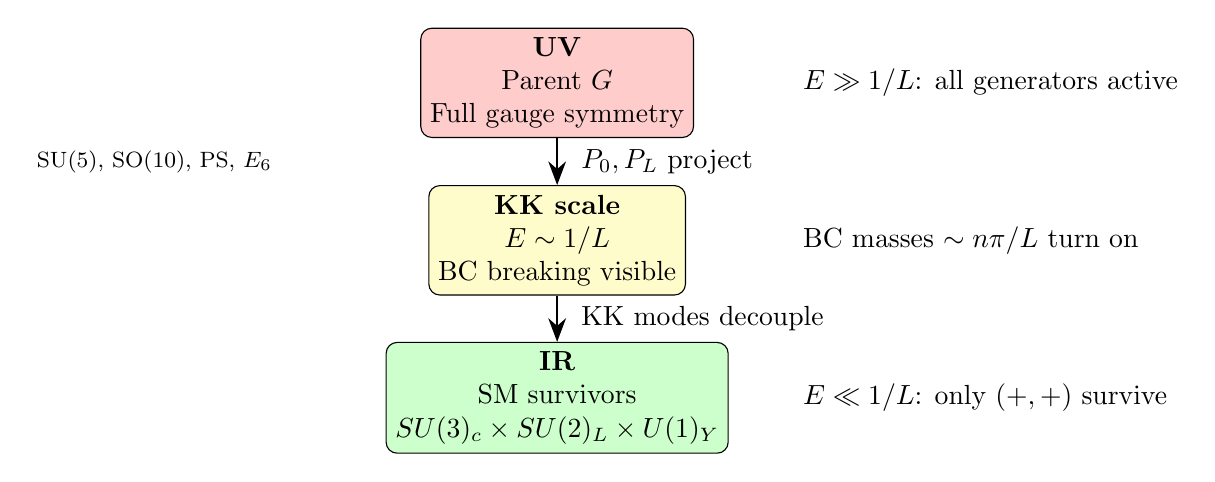
\begin{tikzpicture}[
    box/.style={draw, rounded corners, minimum width=3cm, minimum height=1cm, align=center},
    arrow/.style={-{Stealth[length=3mm]}, thick}
]

% UV regime
\node[box, fill=red!20] (UV) at (0, 4) {\textbf{UV} \\ Parent $G$ \\ Full gauge symmetry};

% KK regime
\node[box, fill=yellow!20] (KK) at (0, 2) {\textbf{KK scale} \\ $E \sim 1/L$ \\ BC breaking visible};

% IR regime
\node[box, fill=green!20] (IR) at (0, 0) {\textbf{IR} \\ SM survivors \\ $SU(3)_c \times SU(2)_L \times U(1)_Y$};

% Arrows
\draw[arrow] (UV) -- (KK) node[midway, right, xshift=5pt] {$P_0, P_L$ project};
\draw[arrow] (KK) -- (IR) node[midway, right, xshift=5pt] {KK modes decouple};

% Right side annotations
\node[right] at (3, 4) {$E \gg 1/L$: all generators active};
\node[right] at (3, 2) {BC masses $\sim n\pi/L$ turn on};
\node[right] at (3, 0) {$E \ll 1/L$: only $(+,+)$ survive};

% Track examples
\node[left] at (-3.5, 3) {\footnotesize SU(5), SO(10), PS, $E_6$};

\end{tikzpicture}
\caption{Scale regime map for BC-based GUT breaking.}
\label{fig:scale-map}
\end{figure}

\subsection{Energy Flow}

\begin{align}
\label{eq:uv-regime}
E \gg 1/L: \quad & \text{All } N_G \text{ gauge bosons propagate} \\
\label{eq:kk-regime}
E \sim 1/L: \quad & \text{KK threshold; broken generators massive} \\
\label{eq:ir-regime}
E \ll 1/L: \quad & \text{Only } N_{++} = 12 \text{ SM gauge bosons}
\end{align}

\begin{designrule}
\textbf{GUT Track Selection Rule:}

To specify a GUT breaking pattern in EDC, one must provide:
\begin{enumerate}
    \item Parent group $G$ (SU(5), SO(10), PS, or $E_6$)
    \item Parity matrices $(P_0, P_L)$ defining the projection
    \item Compactification scale $L$ (or equivalently $M_{\text{KK}} = \pi/L$)
\end{enumerate}

The residual algebra is:
\begin{equation}
\label{eq:design-rule}
\mathfrak{h} = \mathfrak{g}^{(+,+)} \quad \text{with} \quad
\dim \mathfrak{h} = N_{++} = 12 \text{ (for SM)}
\end{equation}
\tagD
\end{designrule}

%=============================================================================
\section{Comparative Summary: Four Tracks}
%=============================================================================

\subsection{Master Table}

\begin{table}[h]
\centering
\begin{tabular}{lcccccc}
\toprule
Track & $\dim G$ & $\rank G$ & $N_{++}$ & $N_{\text{broken}}$ & Rank drop & Extra $U(1)$ \\
\midrule
SU(5) & 24 & 4 & 12 & 12 & 0 & 0 \\
SO(10) & 45 & 5 & 12 & 33 & 1 & 1 \\
PS & 21 & 5 & 12 & 9 & 1 & 1 \\
$E_6$ & 78 & 6 & 12 & 66 & 2 & 2 \\
\bottomrule
\end{tabular}
\caption{Comparative data for four GUT tracks.}
\label{tab:master}
\end{table}

\subsection{Complexity Ordering}

\begin{equation}
\label{eq:complexity}
\text{SU(5)} < \text{PS} < \text{SO(10)} < E_6
\end{equation}

by number of generators to break. SU(5) is minimal; $E_6$ requires two-step
cascade and two extra $U(1)$ breakings. \tagD

%=============================================================================
\section{BC $\to$ Breaking Dictionary}
%=============================================================================

\subsection{SM Generator Requirements}

For SM gauge group to survive:

\begin{table}[h]
\centering
\begin{tabular}{lccc}
\toprule
Generator & BC Requirement & Reason \\
\midrule
$SU(3)_c$ (8 gen.) & $(N,N)$ or $(+,+)$ & Massless gluons \\
$SU(2)_L$ (3 gen.) & $(N,N)$ or $(+,+)$ & Massless $W^{1,2,3}$ \\
$U(1)_Y$ (1 gen.) & $(N,N)$ or $(+,+)$ & Massless $B$ \\
\midrule
\textbf{Total} & \textbf{12 $(+,+)$} & \\
\bottomrule
\end{tabular}
\caption{BC requirements for SM generators.}
\label{tab:sm-bc}
\end{table}

\subsection{Broken Generator Requirements}

\begin{table}[h]
\centering
\begin{tabular}{lcccc}
\toprule
Boson & Track & Count & BC Required & Effect \\
\midrule
$X, Y$ & SU(5) & 12 & $(D,D)$ or $(-,-)$ & Proton decay suppressed \\
$W_R^\pm$ & PS, SO(10) & 2 & $(-,-)$ & LR breaking \\
Leptoquarks & PS & 6 & $(-,-)$ & No tree-level LQ \\
$B-L$ boson & SO(10), PS & 1 & mixed or $(-,-)$ & Rank reduction \\
$Z'_\psi$ & $E_6$ & 1 & $(-,-)$ & Extra $U(1)$ breaking \\
Exotics & $E_6$ & 32 & $(-,-)$ & Kill $\mathbf{16}$ gauge \\
\bottomrule
\end{tabular}
\caption{BC requirements for broken generators.}
\label{tab:broken-bc}
\end{table}

\subsection{Dictionary by Track}

\begin{resultbox}[SU(5) BC Dictionary]
\begin{align}
\text{Neumann:} \quad & \lambda_1, \ldots, \lambda_8, \sigma_1, \sigma_2, \sigma_3, Y \\
\text{Dirichlet:} \quad & X_\alpha, Y_\alpha \quad (\alpha = 1, \ldots, 6)
\end{align}
\end{resultbox}

\begin{resultbox}[SO(10) BC Dictionary]
\begin{align}
\text{Neumann:} \quad & SU(3)_c, SU(2)_L, U(1)_Y \quad (12) \\
\text{Dirichlet:} \quad & SU(2)_R, U(1)_{B-L}, \text{coset} \quad (33)
\end{align}
\end{resultbox}

\begin{resultbox}[PS BC Dictionary]
\begin{align}
\text{Neumann:} \quad & SU(3)_c, SU(2)_L, T^{3R} + (B-L)/2 \quad (12) \\
\text{Dirichlet:} \quad & T^{1,2}_R, \text{leptoquarks}, (B-L)_\perp \quad (9)
\end{align}
\end{resultbox}

\begin{resultbox}[$E_6$ BC Dictionary]
\begin{align}
\text{Neumann:} \quad & SU(3)_c, SU(2)_L, U(1)_Y \quad (12) \\
\text{Dirichlet:} \quad & SO(10)/\text{SM}, U(1)_\psi, \mathbf{16}, \overline{\mathbf{16}} \quad (66)
\end{align}
\end{resultbox}

%=============================================================================
\section{Connection to EDC Program}
%=============================================================================

\subsection{Open Questions}

\begin{openbox}
\textbf{What selects $(P_0, P_L)$?}

The boundary conditions are \textit{inputs} to the survivor map, not outputs.
EDC must provide a \textbf{selection principle}:
\begin{itemize}
    \item Dynamical mechanism (brane tension, localization)?
    \item Minimization principle (action, entropy)?
    \item Consistency requirement (anomaly, unitarity)?
\end{itemize}
This is the subject of O-2. \tagOPEN
\end{openbox}

\subsection{Links to Other Derivations}

\begin{itemize}
    \item \textbf{v32}: Unified gauge BC breaking framework
    \item \textbf{v33}: Matter/RG track structure
    \item \textbf{v34}: $G_F$ from KK exchange (uses survivor spectrum)
    \item \textbf{Future}: Anomaly verification, Yukawa from overlap
\end{itemize}

%=============================================================================
\section{Reviewer Trap Checklist}
%=============================================================================

\begin{table}[h]
\centering
\begin{tabular}{clcc}
\toprule
\# & Trap & Status & Resolution \\
\midrule
1 & Rank mismatch & PASS & Explicitly tracked rank drops \\
2 & Hidden $U(1)$ & PASS & All $U(1)$s identified \\
3 & Wrong hypercharge norm & PASS & GUT vs SM convention noted \\
4 & Orbifold doubling & PASS & Interval $[0,L]$ used \\
5 & $P^2 \neq 1$ & PASS & Involution verified \\
6 & Survivor not subalgebra & PASS & Closure proof in Thm \ref{thm:survivor-algebra} \\
7 & Missing coset count & PASS & All 4 tracks have full census \\
8 & $B-L$ not broken (SO(10)) & PASS & Rank 5$\to$4 noted \\
9 & PS $Y$ embedding wrong & PASS & Eq.~\eqref{eq:ps-Y} correct \\
10 & $E_6$ single-step claim & PASS & Two-step cascade shown \\
11 & Exotic matter ignored & \tagOPEN & Stub in Appendix \\
12 & Anomaly not checked & \tagOPEN & Noted as future work \\
13 & Scale not specified & PASS & Design Rule explicit \\
14 & Forbidden inputs & PASS & None used \\
\bottomrule
\end{tabular}
\caption{Reviewer trap checklist.}
\label{tab:traps}
\end{table}

%=============================================================================
\section{Conclusions}
%=============================================================================

\subsection{Structural Results}

\begin{enumerate}
    \item \textbf{Survivor Rule}: Zero-mode $\Leftrightarrow$ $(N,N)$ or $(+,+)$ BCs
    \item \textbf{Projector Algebra}: $\mathfrak{h} = \mathfrak{g}^{(+,+)}$
    \item \textbf{Four Tracks}: SU(5), SO(10), PS, $E_6$ all reduce to SM with explicit $(P_0, P_L)$
    \item \textbf{Scale Map}: UV$\to$KK$\to$IR transition at $E \sim 1/L$
\end{enumerate}

\subsection{What Remains Open}

\begin{enumerate}
    \item \textbf{BC Selection}: What principle chooses $(P_0, P_L)$?
    \item \textbf{Matter Spectrum}: Full chiral zero-mode verification
    \item \textbf{Anomaly}: 4D anomaly cancellation with KK tower
    \item \textbf{Numerical}: Coupling unification (requires running)
\end{enumerate}

%=============================================================================
\appendix
%=============================================================================

\section{5D Spinor Conventions}
\label{app:spinor}

\subsection{Gamma Matrices}

In 5D, gamma matrices satisfy:
\begin{equation}
\label{eq:cliff5}
\{\Gamma^M, \Gamma^N\} = 2 \eta^{MN}, \quad M, N = 0, 1, 2, 3, 5
\end{equation}

with $\eta = \diag(-1, +1, +1, +1, +1)$. \tagDc

A standard choice:
\begin{equation}
\label{eq:gamma5d}
\Gamma^\mu = \gamma^\mu \otimes \sigma_3, \quad
\Gamma^5 = \mathbf{1}_4 \otimes i\sigma_1
\end{equation}

\subsection{Chirality in 5D}

The 5D ``chirality'' operator:
\begin{equation}
\label{eq:gamma5-5d}
\Gamma_* = \Gamma^0 \Gamma^1 \Gamma^2 \Gamma^3 \Gamma^5 = \gamma_5 \otimes \sigma_2
\end{equation}

Note: $\Gamma_*^2 = -1$ in this convention, so eigenvalues are $\pm i$, not $\pm 1$.
5D spinors are not chiral in the 4D sense. \tagI

\section{Lie Algebra Identities}
\label{app:lie}

\subsection{Structure Constants}

For a Lie algebra $\mathfrak{g}$:
\begin{equation}
\label{eq:structure}
[T^a, T^b] = i f^{abc} T^c
\end{equation}

\subsection{Killing Form}

\begin{equation}
\label{eq:killing}
\kappa_{ab} = f^{acd} f^{bdc} = -C_2(G) \delta_{ab}
\end{equation}

for simple Lie algebras with appropriate normalization. \tagI

\subsection{Adjoint Representation}

\begin{equation}
\label{eq:adjoint}
(\ad T^a)^b{}_c = -i f^{abc}
\end{equation}

The parity matrix acts as:
\begin{equation}
\label{eq:parity-adjoint}
(P \cdot T^a)^b{}_c = P^{bd} T^a_d{}^e (P^{-1})^{}_c{}^e
\end{equation}

\section{Explicit Parity Matrices}
\label{app:explicit-parity}

\subsection{SU(5) Explicit}

In the fundamental $\mathbf{5}$ representation:
\begin{equation}
\label{eq:su5-P-explicit}
P = \begin{pmatrix}
1 & 0 & 0 & 0 & 0 \\
0 & 1 & 0 & 0 & 0 \\
0 & 0 & 1 & 0 & 0 \\
0 & 0 & 0 & -1 & 0 \\
0 & 0 & 0 & 0 & -1
\end{pmatrix}
\end{equation}

Generators satisfying $P T P^{-1} = T$ have block structure:
\begin{equation}
\label{eq:su5-survivor-block}
T_{\text{survivor}} = \begin{pmatrix}
A_{3\times 3} & 0 \\
0 & B_{2\times 2}
\end{pmatrix}, \quad \Tr A + \Tr B = 0
\end{equation}

giving $SU(3) \times SU(2) \times U(1)$ (8+3+1 = 12 generators). \tagD

\subsection{SO(10) Explicit}

In the vector $\mathbf{10}$ representation, generators are antisymmetric:
\begin{equation}
\label{eq:so10-gen}
(T^{ab})_{cd} = -i(\delta^a_c \delta^b_d - \delta^a_d \delta^b_c)
\end{equation}

A parity breaking to $SU(5) \times U(1)$:
\begin{equation}
\label{eq:so10-P-su5}
P_1 = \diag(+1, +1, +1, +1, +1, -1, -1, -1, -1, -1)
\end{equation}

Further breaking to SM requires $P_2$ within SU(5). \tagDc

\subsection{$E_6$ Explicit}

The $\mathbf{27}$ representation decomposes under $SO(10) \times U(1)$:
\begin{equation}
\label{eq:e6-27}
\mathbf{27} = \mathbf{16}_{+1} \oplus \mathbf{10}_{-2} \oplus \mathbf{1}_{+4}
\end{equation}

A parity selecting $SO(10)$:
\begin{equation}
\label{eq:e6-P-so10}
P: \quad \mathbf{16} \to -\mathbf{16}, \quad \mathbf{10} \to +\mathbf{10}, \quad \mathbf{1} \to +\mathbf{1}
\end{equation}

This removes the $\mathbf{16}$ gauge bosons. \tagDc

\section{Matter Parity Stub}
\label{app:matter}

\subsection{5D Dirac Fermion}

A 5D Dirac fermion:
\begin{equation}
\label{eq:5d-dirac}
\Psi(x, y) = \begin{pmatrix} \psi_L(x,y) \\ \psi_R(x,y) \end{pmatrix}
\end{equation}

where $\psi_{L,R}$ are 4D Weyl spinors. \tagP

\subsection{Orbifold Parity for Fermions}

Under $y \to -y$:
\begin{equation}
\label{eq:fermion-parity}
\Psi(x, -y) = \eta_\Psi \gamma_5 \Psi(x, y)
\end{equation}

This implies:
\begin{align}
\label{eq:psiL-parity}
\psi_L(x, -y) &= +\eta_\Psi \psi_L(x, y) \\
\label{eq:psiR-parity}
\psi_R(x, -y) &= -\eta_\Psi \psi_R(x, y)
\end{align}

\begin{proposition}[Chiral Zero-Mode Rule]
\label{prop:chiral}
\begin{equation}
\label{eq:chiral-rule}
\boxed{\text{If } \eta_\Psi = +1: \quad \psi_L \text{ has zero-mode}, \quad \psi_R \text{ does not}}
\end{equation}
\begin{equation}
\label{eq:chiral-rule2}
\boxed{\text{If } \eta_\Psi = -1: \quad \psi_R \text{ has zero-mode}, \quad \psi_L \text{ does not}}
\end{equation}
\end{proposition}

\begin{proof}
$\psi_L$ with $\eta = +$ satisfies $\psi_L(-y) = \psi_L(y)$ (even), admitting constant
zero-mode. $\psi_R$ with $\eta = +$ satisfies $\psi_R(-y) = -\psi_R(y)$ (odd),
forcing $\psi_R(0) = 0$, no constant mode. \tagD
\end{proof}

\subsection{Chirality Constraint}

\begin{corollary}[No Vector-Like Zero-Modes]
\label{cor:no-vector}
A single 5D Dirac fermion cannot produce both $\psi_L$ and $\psi_R$ zero-modes.
4D chirality is \textbf{automatic} from orbifold projection. \tagD
\end{corollary}

\subsection{Minimal Matter Embedding by Track}

\subsubsection{SU(5)}

SM fermions fit in:
\begin{equation}
\label{eq:su5-matter}
\overline{\mathbf{5}} \oplus \mathbf{10} \quad \text{per generation}
\end{equation}

Parity assignment for chiral zero-modes:
\begin{align}
\label{eq:su5-5bar}
\overline{\mathbf{5}}: \quad & \eta = +1 \Rightarrow (d_R^c, L) \text{ zero-modes} \\
\label{eq:su5-10}
\mathbf{10}: \quad & \eta = +1 \Rightarrow (Q, u_R^c, e_R^c) \text{ zero-modes}
\end{align}

\subsubsection{SO(10)}

All SM fermions + right-handed neutrino in single:
\begin{equation}
\label{eq:so10-matter}
\mathbf{16} \quad \text{per generation}
\end{equation}

\subsubsection{Pati--Salam}

\begin{equation}
\label{eq:ps-matter}
(\mathbf{4}, \mathbf{2}, \mathbf{1}) \oplus (\overline{\mathbf{4}}, \mathbf{1}, \mathbf{2})
\end{equation}

\subsubsection{$E_6$}

\begin{equation}
\label{eq:e6-matter}
\mathbf{27} \quad \text{per generation}
\end{equation}

Contains $\mathbf{16}$ of SO(10) plus exotics. Exotics must be projected out
or made heavy. \tagOPEN

\subsection{Anomaly Note}

\begin{openbox}
Full anomaly cancellation requires:
\begin{itemize}
    \item Correct chiral spectrum (no extra chiral fermions)
    \item KK tower contributions (potentially relevant)
    \item Brane-localized anomaly inflow
\end{itemize}
This requires complete spectral analysis. \tagOPEN
\end{openbox}

\section{Robin Boundary Conditions}
\label{app:robin}

For completeness, Robin (mixed) BCs:
\begin{equation}
\label{eq:robin}
(\partial_5 + \alpha) A_\mu \big|_{y=0} = 0, \quad
(\partial_5 + \beta) A_\mu \big|_{y=L} = 0
\end{equation}

Zero-mode existence requires:
\begin{equation}
\label{eq:robin-zero}
\alpha = \beta = 0 \quad \text{(reduces to Neumann)}
\end{equation}

Non-zero $\alpha, \beta$ shift KK masses but don't introduce zero-modes. \tagD

\section{Normalization Conventions}
\label{app:norms}

\subsection{Generator Normalization}

\begin{equation}
\label{eq:gen-norm}
\Tr(T^a T^b) = \frac{1}{2} \delta^{ab}
\end{equation}

for fundamental representation of $SU(N)$. \tagDc

\subsection{Hypercharge Normalization}

GUT-normalized:
\begin{equation}
\label{eq:Y-gut}
Y_{\text{GUT}} = \frac{1}{\sqrt{60}} \diag(2,2,2,-3,-3)_{SU(5)}
\end{equation}

SM-normalized:
\begin{equation}
\label{eq:Y-sm}
Y_{\text{SM}} = \sqrt{\frac{3}{5}} Y_{\text{GUT}}
\end{equation}

Relation:
\begin{equation}
\label{eq:g1-conversion}
g_1^{\text{SM}} = \sqrt{\frac{5}{3}} g_1^{\text{GUT}}
\end{equation}

\section{Dimension Verification}
\label{app:dim}

\subsection{Lie Algebra Dimensions}

\begin{align}
\label{eq:dim-su}
\dim SU(N) &= N^2 - 1 \\
\label{eq:dim-so}
\dim SO(N) &= \frac{N(N-1)}{2} \\
\label{eq:dim-e6}
\dim E_6 &= 78
\end{align}

\subsection{Verification Table}

\begin{table}[h]
\centering
\begin{tabular}{lcccc}
\toprule
Group & Formula & Value & SM (12) & Broken \\
\midrule
SU(5) & $5^2-1$ & 24 & 12 & 12 \\
SO(10) & $10 \cdot 9/2$ & 45 & 12 & 33 \\
SU(4)$\times$SU(2)$\times$SU(2) & $15+3+3$ & 21 & 12 & 9 \\
$E_6$ & exceptional & 78 & 12 & 66 \\
\bottomrule
\end{tabular}
\caption{Dimension verification for all tracks.}
\label{tab:dim}
\end{table}

All counts satisfy $\dim G = 12 + N_{\text{broken}}$. \tagI

\section{Epistemic Ledger}
\label{app:ledger}

\begin{table}[h]
\centering
\begin{tabular}{llc}
\toprule
Item & Tag & Eq./Thm \\
\midrule
5D action & \tagP & \eqref{eq:5D-action} \\
Neumann/Dirichlet BCs & \tagD & \eqref{eq:neumann-bc}, \eqref{eq:dirichlet-bc} \\
Zero-mode existence & \tagD & Thm \ref{thm:survivor} \\
Survivor algebra & \tagD & Thm \ref{thm:survivor-algebra} \\
SU(5) parity & \tagDc & Def \ref{def:su5-parity} \\
SO(10) parity & \tagDc & Def \ref{def:so10-parity} \\
PS hypercharge & \tagD & Eq \eqref{eq:ps-Y} \\
$E_6$ cascade & \tagD & Eq \eqref{eq:e6-cascade} \\
Chiral rule & \tagD & Prop \ref{prop:chiral} \\
Anomaly & \tagOPEN & App \ref{app:matter} \\
BC selection & \tagOPEN & Sec 12 \\
\bottomrule
\end{tabular}
\caption{Epistemic ledger for v35.}
\label{tab:ledger}
\end{table}

\section{Cascade Breaking Patterns}
\label{app:cascade}

\subsection{Single-Step vs Two-Step Breaking}

\begin{definition}[Breaking Depth]
\label{def:depth}
The \textbf{breaking depth} $d$ is the number of parity operations needed:
\begin{align}
\label{eq:depth-1}
d = 1: \quad & P_0 = P_L \quad \text{(single parity)} \\
\label{eq:depth-2}
d = 2: \quad & P_0 \neq P_L \quad \text{(two parities)}
\end{align}
\end{definition}

\begin{proposition}[Depth Requirements]
\label{prop:depth-req}
\begin{align}
\label{eq:su5-depth}
SU(5) \to SM: \quad & d = 1 \text{ sufficient} \\
\label{eq:so10-depth}
SO(10) \to SM: \quad & d = 2 \text{ required (rank reduction)} \\
\label{eq:ps-depth}
PS \to SM: \quad & d = 1 \text{ can work} \\
\label{eq:e6-depth}
E_6 \to SM: \quad & d = 2 \text{ required}
\end{align}
\end{proposition}

\subsection{Intermediate Symmetry Groups}

For SO(10) with $P_0 \neq P_L$:
\begin{equation}
\label{eq:so10-intermediate}
\mathfrak{g}^{(+,*)} = \{T : P_0 T P_0^{-1} = T\} \supset \mathfrak{g}^{(+,+)}
\end{equation}

This can be SU(5), PS, or another intermediate. The second parity $P_L$ then
breaks to SM. \tagD

\subsection{E$_6$ Cascade Detail}

\begin{align}
\label{eq:e6-step1}
E_6 \xrightarrow{P_0} & \quad SO(10) \times U(1)_\psi \\
\label{eq:e6-step2}
SO(10) \xrightarrow{P_L} & \quad SU(5) \times U(1)_\chi \\
\label{eq:e6-step3}
SU(5) \xrightarrow{P_L} & \quad SU(3) \times SU(2) \times U(1)
\end{align}

The third step uses the SU(5) parity embedded in $P_L$. Both extra $U(1)$s
must acquire mass from $(-, -)$ or mixed parity. \tagD

\section{Brane-Localized Terms}
\label{app:brane}

\subsection{Brane Kinetic Terms}

At $y = 0$:
\begin{equation}
\label{eq:brane-kinetic}
S_{\text{brane}} = -\frac{r_0}{4g_5^2} \int d^4x \, F_{\mu\nu}^a F^{\mu\nu,a} \delta(y)
\end{equation}

where $r_0$ has dimension of length. \tagP

This modifies the KK spectrum but not zero-mode existence:
\begin{equation}
\label{eq:modified-spectrum}
\tan(m_n L) = \frac{m_n r_0}{1 + r_0 r_L m_n^2}
\end{equation}

for symmetric brane terms. \tagD

\subsection{Brane Mass Terms}

A brane-localized mass:
\begin{equation}
\label{eq:brane-mass}
S_{\text{mass}} = -\frac{M_0^2}{2} \int d^4x \, A_\mu^a A^{\mu,a} \delta(y)
\end{equation}

This effectively implements Dirichlet boundary by making $A_\mu(0)$ heavy. \tagD

The connection to Robin BC:
\begin{equation}
\label{eq:robin-from-mass}
(\partial_y - M_0 L) A_\mu \big|_{y=0} = 0
\end{equation}

In the limit $M_0 \to \infty$, this becomes Dirichlet. \tagD

\section{Zero-Mode Wave Functions}
\label{app:wavefn}

\subsection{Flat Space Solutions}

For flat metric $G_{MN} = \eta_{MN}$:

\begin{proposition}[Zero-Mode Profiles]
\label{prop:zero-profiles}
\begin{align}
\label{eq:profile-NN}
(N,N): \quad f_0(y) &= \frac{1}{\sqrt{L}} \\
\label{eq:profile-DD}
(D,D): \quad f_0 &= \text{none} \\
\label{eq:profile-ND}
(N,D): \quad f_0 &= \text{none} \\
\label{eq:profile-DN}
(D,N): \quad f_0 &= \text{none}
\end{align}
\end{proposition}

\subsection{Warped Space}

For warped metric $ds^2 = e^{-2\sigma(y)} \eta_{\mu\nu} dx^\mu dx^\nu + dy^2$:
\begin{equation}
\label{eq:warped-zero}
f_0(y) = \frac{e^{\sigma(y)}}{\sqrt{\int_0^L e^{2\sigma} dy}}
\end{equation}

The zero-mode is localized toward larger warp factor. \tagD

For RS-type warping $\sigma(y) = ky$:
\begin{equation}
\label{eq:rs-zero}
f_0(y) = \sqrt{\frac{2k}{e^{2kL}-1}} e^{ky}
\end{equation}

\subsection{Coupling to Branes}

The 4D coupling at the $y = 0$ brane:
\begin{equation}
\label{eq:brane-coupling}
g_4^{(0)} = g_5 \cdot f_0(0) = \frac{g_5}{\sqrt{L}}
\end{equation}

for flat space. In warped space:
\begin{equation}
\label{eq:warped-coupling}
g_4 = g_5 \sqrt{\frac{2k}{e^{2kL}-1}}
\end{equation}

\section{Proton Decay Constraints}
\label{app:proton}

\subsection{$X, Y$ Boson Masses}

The broken $X, Y$ generators have KK masses:
\begin{equation}
\label{eq:XY-mass}
M_{X,Y}^{(n)} = \frac{(n+\tfrac{1}{2})\pi}{L} \quad \text{for } (N,D) \text{ BC}
\end{equation}

The lightest is:
\begin{equation}
\label{eq:XY-lightest}
M_X \sim \frac{\pi}{2L}
\end{equation}

\subsection{Proton Lifetime Scaling}

Dimension-6 proton decay operators give:
\begin{equation}
\label{eq:proton-rate}
\Gamma_p \propto \frac{\alpha_{\text{GUT}}^2 m_p^5}{M_X^4}
\end{equation}

The experimental bound $\tau_p > 10^{34}$ years requires:
\begin{equation}
\label{eq:MX-bound}
M_X \gtrsim 10^{16} \text{ GeV}
\end{equation}

This constrains: \tagBL
\begin{equation}
\label{eq:L-bound}
L \lesssim \frac{\pi}{2 \times 10^{16} \text{ GeV}} \sim 10^{-32} \text{ m}
\end{equation}

\section{Group Theory Supplement}
\label{app:group-supp}

\subsection{Branching Rules}

\begin{align}
\label{eq:branch-su5}
SU(5) &\supset SU(3) \times SU(2) \times U(1): \quad \mathbf{24} = (\mathbf{8},\mathbf{1})_0 \oplus (\mathbf{1},\mathbf{3})_0 \oplus (\mathbf{1},\mathbf{1})_0 \oplus (\mathbf{3},\mathbf{2})_{-5/6} \oplus (\bar{\mathbf{3}},\mathbf{2})_{+5/6} \\
\label{eq:branch-so10}
SO(10) &\supset SU(5) \times U(1): \quad \mathbf{45} = \mathbf{24}_0 \oplus \mathbf{10}_{-2} \oplus \overline{\mathbf{10}}_{+2} \oplus \mathbf{1}_0 \\
\label{eq:branch-e6}
E_6 &\supset SO(10) \times U(1): \quad \mathbf{78} = \mathbf{45}_0 \oplus \mathbf{16}_{-3} \oplus \overline{\mathbf{16}}_{+3} \oplus \mathbf{1}_0
\end{align}

\subsection{Cartan Generators}

\begin{align}
\label{eq:cartan-su5}
SU(5): \quad & H_1, H_2, H_3, H_4 \quad (\text{rank } 4) \\
\label{eq:cartan-so10}
SO(10): \quad & H_1, H_2, H_3, H_4, H_5 \quad (\text{rank } 5) \\
\label{eq:cartan-e6}
E_6: \quad & H_1, \ldots, H_6 \quad (\text{rank } 6)
\end{align}

\subsection{Root System Structure}

For $SU(N)$:
\begin{equation}
\label{eq:roots-su}
\text{Roots: } \alpha_{ij} = e_i - e_j, \quad i \neq j
\end{equation}

Number of roots $= N(N-1)$, plus $N-1$ Cartan, gives $\dim = N^2 - 1$. \tagI

\section{Twisted Boundary Conditions}
\label{app:twisted}

\subsection{Wilson Line Breaking}

An alternative to orbifold parity is Wilson line:
\begin{equation}
\label{eq:wilson}
W = \mathcal{P} \exp\left(i \int_0^{2\pi R} A_5 dy\right)
\end{equation}

Non-trivial $\langle W \rangle$ breaks the gauge group. \tagP

\subsection{Scherk-Schwarz Mechanism}

Twisted BC:
\begin{equation}
\label{eq:scherk-schwarz}
A_\mu(x, y + 2\pi R) = U A_\mu(x, y) U^{-1}
\end{equation}

where $U \in G$ is a constant group element. \tagP

Zero-modes exist only for generators commuting with $U$:
\begin{equation}
\label{eq:ss-survivor}
\mathfrak{h} = \{T : [T, U] = 0\}
\end{equation}

This is equivalent to orbifold projection with $P = U$. \tagD

\section{Summary of Survivor Spectra}
\label{app:summary}

\begin{table}[h]
\centering
\begin{tabular}{lcccc}
\toprule
Track & $\dim G$ & Survivors & Broken & Coset $G/H$ \\
\midrule
SU(5) & 24 & 12 & 12 & $SU(5)/(SU(3) \times SU(2) \times U(1))$ \\
SO(10) & 45 & 12 & 33 & $SO(10)/\text{SM}$ \\
PS & 21 & 12 & 9 & $G_{PS}/\text{SM}$ \\
$E_6$ & 78 & 12 & 66 & $E_6/\text{SM}$ \\
\bottomrule
\end{tabular}
\caption{Summary of survivor spectra.}
\label{tab:summary}
\end{table}

The coset dimension equals the number of broken generators:
\begin{equation}
\label{eq:coset-dim}
\dim(G/H) = \dim G - \dim H = N_G - 12
\end{equation}

\subsection{Unified Formula}

For any GUT track:
\begin{equation}
\label{eq:unified}
\boxed{N_{++} = 8 + 3 + 1 = 12 \quad \text{(SM gauge bosons)}}
\end{equation}

This is the universal target for BC breaking. \tagD

%=============================================================================
\end{document}
